\section{Usage}
\suppressfloats[t]

Depending on whether you are constructing a graph production system which
should be visualised and simulated, or are analyzing an existing production
system, you will need a good user interface or be content with a command-line
tool that is optimised for performance. For the first purpose, the GROOVE
tool set includes the Editor and Simulator tools; for the latter, the Generator 
and ModelChecker.

\subsection{Editor}

We will first discuss the Editor as a stand-alone tool. Note, however, that it
can also be invoked from the Simulator; in fact, we expect this to be the more
usual way of working.

The Editor is a rather primitive tool; in particular, while editing the
special coloured representation of rule elements (erasers, embargoes etc) and
data values (ellipsoid and diamond-shaped nodes) are not available. Instead
these features have to be encoded through \emph{prefixes}.

\subsubsection{Rules and data values}

\subsubsection{Actions}

\begin{table}
\begin{center}
\begin{tabular}{|p{5cm}|p{8cm}|}
\hline\hline
\bf Action & \bf Description \\
\hline
\bf Add Point
 & Adds an intermediate point to the currently selected edge, through which it
 can be routed. \\
\bf Edit Properties
 & Calls up a dialog in which graph properties can be added, changed or
 deleted. These can be user-defined properties but include \texttt{priority}
 and \texttt{enabled}; both refer to the case where the graph is used as a
 production rule. \\
\bf Options 
 & Calls up a menu with behavioural and display options. \\
\bf Remove Point
 & \\
\bf Reset Label
 & Sets the labels of the currently selected edges to their default positions \\
\bf Set Line Style
 & Changes the line style of the currently selected edges \\
\hline\hline
\end{tabular}
\end{center}
\caption{Editor actions}
\end{table}


\subsection{Simulator}

\subsubsection{Panels}

\paragraph{Graph panel}

\paragraph{Rule panel}

\paragraph{LTS panel}

\subsubsection{Visualisation options}

\paragraph{Emphasising}

\paragraph{Graying out}

\paragraph{Filtering}

\subsubsection{Actions}

\subsection{Generator}

\subsubsection{Options}

\paragraph{Hiding and emphasis.}

Both the editor and the simulator of the GROOVE tool set use further visual
tricks to control the display of large graphs: elements of the graphs can be
\emph{hidden} or \emph{emphasized}. 

A hidden node or edge is ``grayed out'': its existence can still be guessed at
from the display but details are obscured. Hiding follows the graph structure,
in the sense that the incoming and outgoing edges of a hidden node are also
automatically hidden. Hiding is entirely user-controlled: parts of a graph can
be hidden, based on labels, manual selection, or regular expressions over edge
labels denoting paths through the graph. (Regular expressions are discussed in
\stref{regexp} below, albeit in the context of rule application rather than
hiding; however, the syntax is the same in both cases.) The graph layouting
algorithms in GROOVE ignore the hidden elements and only affect the visible
part of the graph.

An emphasized node or edge gets a fatter (out)line, and the text is displayed
in bold font. Emphasis does not follow the graph structure. Hidden graph
elements can in fact be emphasized as well, but this is hardly visible.
Emphasis can either be set manually on a label-by-label basis, or is in some
cases set automatically to show the subgraph in which a given rule applies.

For instance, in \fref{emphasis}, the left hand side shows a structure
modelling a circular buffer of three cells, in which one cell holds a value. On
the right hand side, the \Buffer-labelled node has been hidden (automatically
hiding its outgoing \First- and \Last-edges as well) and the \Val- and
\Next-labelled edges have been emphasized.

\texfig{emphasis}{Hiding and emphasis in graphs.}

\subsubsection{Production rules}

\subsubsection{Transition systems}

A \emph{transition system} is a third kind of graph, created as the result of
the simulation of a graph production system. In contrast to the graphs
discussed above, where the elements can be used to model arbitrary concepts and
relations, a transition system is a dedicated kind of graph: the nodes stand
for states and the edges for transitions, which correspond to production rule
applications.

This is not the place to discuss transition systems in detail. See, for
instance, \cite{Rensink2003a} for a discussion of the theoretical background of the
functionality of GROOVE. Here it should suffice to understand that to every
state (i.e., node of the transition system) there is an associated graph, and
to every transition (i.e., edge of the transition system) there is an
associated rule application, which identifies a sub-graph of the source graph
of the transition where the rule can be applied.

In displaying a transition system, we use visual elements for the
following concepts.

\paragraph{State identifiers.}

In contrast to ordinary graphs, in transition systems we do not use node labels
to model self-edges: instead, they reflect the identity of the state. This is
typically just a number, but it provides a way to refer to individual
states. To indicate visually that the node labels have a different
interpretation, they are displayed in italic font.

\paragraph{Transition labels.}

As stated above, to each transition there is an associated rule as well as a
matching of that rule in the source graph; i.e., a sub-graph of the source
graph where the rule is applicable. As transition labels we use the rule names
of the associated rules. To indicate visually that these names are not ordinary
labels we enclose them in triangular brackets; hence, a transition that models
the application of a rule named \textsf{assign} would be labelled
\textsf{$\langle$assign$\rangle$}.

It should be noted that this may result in a seeming contradiction to the
principle, stated above, that no two equally labelled edges may exist between
the same source and target nodes. It is possible that the same rule, applied to
two different sub-graphs of a given graph, results in the same (or more
precisely, isomorphic) target graphs, which in the GROOVE simulation would be
modelled by the same target state of the transition system. Thus, given the
fact that we are using only the rule name as label, this gives rise to two
equally labelled transitions between the same source and target states.

\paragraph{The initial state.}

The simulation of a graph production system always starts in one initial graph,
which gives rise to a unique initial state of the transition system. Since it
is often interesting to keep track of this initial state, we indicate it
visually by giving it a special background colour (namely, green).

\paragraph{Final states.}

Depending on the production system in question, it may be possible to produce a
graph to which no more rules are applicable. Such a \emph{final state} is often
interesting, for instance because it models a desired result or because it
corresponds to an error in the model. Final states are indicated visually by a
special background colour (namely, red).

\paragraph{Open states.}

The transition system resulting from the application of a production system to
a given initial graph is built up step by step. Every step consists of
investigating all possible rule applications in a given graph. We call this
process the \emph{closure} of that state, and states that have not yet been
closed are called \emph{open}. We indicate open states visually by a gray
background colour.

\paragraph{Active state and transition.}

At any point during the process of graph transformation, the GROOVE
simulator is focussed upon a certain graph, and possibly a production rule
that can be applied to that graph. In terms of the transition system, this
gives rise to an \emph{active} state, and possibly an active outgoing
transition of that state. These are indicated visually by a special line
colour (namely, blue).

\texfig{ltss}{An incomplete and a completely explored LTS for the circular
buffer of \fref{emphasis}, using the rules of \fref{circular-display}.}

For instance, \fref{ltss} shows two labelled transition systems, obtained by
applying the rules of \fref{circular-display} to the state on the left hand
side of \fref{emphasis}. In fact, the nodes \emph{s5}, \emph{s6} and \emph{s8}
of \fref{ltss} correspond to the top, right hand, and bottom graphs of
\fref{circular-states}, respectively.

State \emph{s5} is the initial state in both systems. On the left hand side,
state \emph{s8} is open, whereas on the right hand side it is closed.  On the
left hand side there is an active state and on the right hand side an active
transition. Neither transition system has a final state.

\subsection{Regular expressions and node merging}
\stlabel{regexp}

In this section we discuss some special types of labels that can be used in
production rules.

\paragraph{Regular expression labels.}

As we have seen in \stref{rule-display}, reader and embargo edges impose
conditions upon the applicability of rules, rather than controlling the
deletion or creation of graph elements. The succinctness and expressiveness of
such conditions can be enhanced by using \emph{regular expressions} as reader
or embargo edge labels. For instance, to express the condition that two nodes
are connected through some sequence of \nextL-labelled edges, one can use a
reader edge labelled \l{next*}.

In fact, GROOVE supports regular expressions with the operators in
\tref{regexp}. Concatenation has higher priority than choice and the postfix
operators have higher priority still. Ordinary parentheses are used to override
priorities; however, other bracket pairs are also recognized and are required
to be nested properly. Because this obviously limits the set of strings that
can be used as proper labels, GROOVE interprets all singly-quoted subexpressions on
rule labels literally; hence, a label containing a ``forbidden'' character can
be specified by putting single quotes around it.

It should be noted that regular expression labels are only allowed on reader
and embargo edges of production rule graphs: on eraser and creator edges they
are forbidden. In state graphs, on the other hand, no attempt is made to
interpret a label as a regular expression, but proper bracket nesting and quote
usage are nevertheless required.
%
\begin{table}
\begin{center}
\begin{tabular}{|c|l|}
\hline\hline
\bf Expression & \bf Meaning \\
\hline
$'\expL'$ & matches $\expL$ (interpreted as a literal label) \\
$=$ & matches the empty path (equality constraint) \\
$?$ & matches an arbitrary label (wildcard) \\
\hline
$\pathL_1|\pathL_2$ & matches either $\pathL_1$ or $\pathL_2$ \\
$\pathL_1.\pathL_2$ & matches concatenation of $\pathL_1$ and $\pathL_2$ \\
\hline
$\pathL{*}$ & matches zero or more concatenated occurrences of $\pathL$ \\
$\pathL{+}$ & matches one or more concatenated occurrences of $\pathL$ \\
%$\pathL{?}$ & matches zero or one occurrence of $\pathL$ \\
\hline
$(\pathL)$ & matches the same as $\pathL$ \\
\hline
\hline\hline
\end{tabular}
\end{center}
\caption{Special labels.}
\tlabel{regexp}
\end{table}

\paragraph{Inequality contraints.}

Although, as shown in \tref{regexp}, the equality sign $=$ is a special kind of
regular expression, it is used most commonly in isolation, on embargo edges
between reader nodes. Its natural interpretation is then to ensure that the
source and target nodes of such an edge are distinct; that is, the rule will
only be applicable when the source and target nodes correspond to distinct
parts of the graph under transformation.

\paragraph{Node mergers.}

Another use of $=$ as an edge label in rules is on creator edges. This is
distinct from its use in regular expressions, since as stated above, general
regular expressions are forbidden on creator edges. An $=$ label on a creator
edge stands for a \emph{node merger}: the application of such a rule to a given
graph will merge two distinct nodes into one, which will receive all incoming
and outgoing edges of the original nodes. Edges that originally
occurred between the merge nodes will become self-edge of the
resulting node.

\subsection{Attributed graphs}

In this section we will discuss how to enrich graphs with nodes
representing data values (so called \emph{attributed graphs}) and how
to specify production rules in that case. We will explain the use of
these data types by using a simple example.

\paragraph{Build-in data types.}

Currently, we have implemented three basic data types:
\emph{integer}, \emph{boolean}, and \emph{string}. For the integer
data type we have implemented the following operations: $+$ (addition),
$-$ (substraction), $*$ (multiplication), $/$ (division), $\%$
(modulo), $<$ (less than), $>$ (greater) than, and $=$ (equal); for
strings we only support $+$ (concatenation) and $=$ (equals); for
booleans we have implemented $\wedge$ (conjunction), $\vee$
(disjunction), and $\neg$ (negation).

\paragraph{Example graph.}

As an example attributed graph, \fref{algebra-buffer-state} shows a graph
representation of an empty buffer where the slots are identified by
indices. The indices are constant data values from the integer data
type. The buffer also has a \current-attribute referring to the index
of the current slot. It also has a \capacity-attribute which points to
the constant data value indicating the number of slots of this
buffer.

\texfig{algebra-buffer-state}{Empty buffer with capacity 4.}

\paragraph{Example production rule.}

\fref{algebra-buffer-transformation-output} shows a production rule which can
be applied on the buffer from \fref{algebra-buffer-state}. This rule
is only applicable if the \bufferIndex{} of the \current{} cell is less than
the \capacity{} of the buffer, i.e. $\intLT(\current,\capacity) =
\true$. If this rule is applied, the cell with \bufferIndex{}
$\current + 1$ will be attached a fresh created \Object{} and will
become the \current{} cell.

\texfig{algebra-buffer-transformation-output}{Production rule for the buffer
  with indices.}

\paragraph{General principles.} In the production rule we can
distinguish two different ways of using attribute values: (1) as
\emph{input} or as (2) \emph{output} of a specific operation. An
example of the first case is shown in \fref{update}: the current value
serves as input for calculating the new value. In the second case
(see e.g. \fref{condition}), the result of applying the specified
operation on the current values of the attributes should equal the
specified output (or result): the data value determines the
applicability of the rule.

\begin{figure}[htbp]
\begin{center}
\subfigure[Input]{
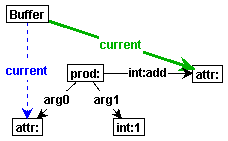
\includegraphics{\figdir/update}
\flabel{update}
}
\subfigure[Output]{
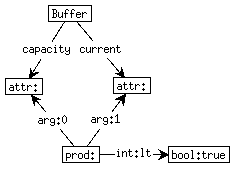
\includegraphics{\figdir/condition}
\flabel{condition}
}
\caption{Using attribute values.}
\flabel{attribute-usage}
\end{center}
\end{figure}

\subsection{Editor format}
\stlabel{input}

The visual formatting of attributed graphs, production rules, and
labelled transition systems, described in the previous section, is the
\emph{display format}. In the editor of the GROOVE tool and for the
purpose of serialising and exchanging production rules, we need a
textual representation of this format. This is true for all of them.

\subsubsection{Attributed graphs}

\fref{algebra-buffer-state} shows the display format of the attributed
graph as well as the editor format. From that figure we want to
address how to include constant data values from different data
types. The general rule is to encode data values as labels of
self-edges of the node representing the data value. These labels are
then of the form: \prefix:\constantSymbol, where \prefix{} must be
replaced by one of the prefixes listed in \tref{data-types} and
\constantSymbol{} by a textual representation of the actual data
value.\footnote{In the GXL format the self-edge of nodes representing
  data values is stored as a simple edge with the entire label. In the
  near future we plan to use GXL-specific encodings for this in order
  to make the graph exported by GROOVE easier to process by other
  tools.} Some examples are given in \tref{algebra-values}.

\begin{table}[htbp]
  \centering
  \begin{tabular}{|c|c|}
  \hline\hline
  {\bf Data Type} & {\bf Prefix} \\
  \hline
  Integer & \texttt{int} \\
  String & \texttt{string} \\
  Boolean & \texttt{bool} \\
  \hline\hline
  \end{tabular}
  \caption{Data types with their corresponding prefixes.}
  \tlabel{data-types}
\end{table}

\begin{table}[htbp]
  \centering
  \begin{tabular}{|c|c|}
  \hline\hline
  {\bf Data Value} & {\bf Editor Format} \\
  \hline
  integer 1 & \texttt{int:1} \\
  string ``hello'' & \texttt{string:hello} \\
  boolean \true & \texttt{bool:true} \\
  \hline\hline
  \end{tabular}
  \caption{Data values with their corresponding editor format.}
  \tlabel{algebra-values}
\end{table}

\subsubsection{Production rules}

In particular, we need a way to categorise rule
nodes and edges as reader, eraser, embargo or creator. This is done by
introducing special \emph{role prefixes}, listed in \tref{prefixes}.
%
\begin{table}[htbp]
\begin{center}
\begin{tabular}{|c|l|}
\hline\hline
\bf Prefix & \bf Meaning \\
\hline
\emph{(none)} & Reader node or edge \\
\Use & Reader node or edge \\
\Del & Eraser node or edge \\
\Not & Embargo node or edge (incl.\ merge embargo) \\
\New & Creator node or edge (incl.\ merger) \\
\hline
\Start & Start node of a labelled transition system \\
\Final & Final node of a labelled transition system \\
\Open & Open node of a labelled transition system \\
\hline\hline
\end{tabular}
\end{center}
\caption{Role prefixes in the editor format for production rules and labelled
transition systems.}
\tlabel{prefixes}
\end{table}
%
For nodes, the role is indicated by a special self-edge labeled exclusively by
the role prefix; for edges, the prefix is inserted in front of the edge label.
Note that reader elements do not necessarily need a role prefix: the absence of
any prefix indicates a reader node or edge. Furthermore, for edges incident to
eraser, embargo or creator nodes the role prefix can be left out, since it is
implicit.
%
\texfig{rule-input}{
    The rules of Figures~\ref{f:append-rule} and \ref{f:assign-rule} in editor
    format.
}%
%
As an example, \fref{rule-input} shows the production rules of
Figures~\ref{f:append-rule} and \ref{f:assign-rule} in editor format.
\fref{circular-input} shows the editor format of the rules in
\fref{circular-display}.
%
\texfig{circular-input}{The production rules \Put{} and \Get{} of
  \fref{circular-display} in editor format.}

When specifying production rules over attributed graphs, we need to
introduce a way to refer to algebraic operations to be applied on
particular data values. Since we cannot assume that every operation
(no matter from which data type) has a distinct symbol, we need an
editor format comparable to the one used for data values:
\prefix:\operationSymbol, where \operationSymbol{} must be replaced by
the textual representations of the specific algebraic operation, as
listed in \tref{algebra-operations}.

\begin{table}[htbp]
  \centering
  \begin{tabular}{|c|c|c|}
  \hline\hline
  {\bf Data Type} & {\bf Operation Symbol} & {\bf Editor Format} \\
  \hline
  \multirow{8}*{Integer} & $+$  & \texttt{add} \\
                         & $-$  & \texttt{sub} \\
                         & $*$  & \texttt{mul} \\
                         & $/$  & \texttt{div} \\
                         & $\%$ & \texttt{mod} \\
                         & $=$  & \texttt{eq} \\
                         & $<$  & \texttt{lt} \\
                         & $<=$  & \texttt{le} \\
                         & $>$  & \texttt{gt} \\
                         & $>=$  & \texttt{ge} \\
  \hline
  \multirow{2}*{String}  & $+$  & \texttt{concat} \\
                         & $=$  & \texttt{eq} \\
  \hline
  \multirow{2}*{Boolean} & $\wedge$ & \texttt{and} \\
                         & $\vee$   & \texttt{or} \\
                         & $\neg$   & \texttt{not} \\
  \hline\hline
  \end{tabular}
  \caption{Algebraic operations with their corresponding editor format.}
  \tlabel{algebra-operations}
\end{table}

\fref{algebra-buffer-transformation-input} shows the editor format of
the production rule from \fref{algebra-buffer-transformation-output}.

\texfig{algebra-buffer-transformation-input}{Editor format of the
  production rule from \fref{algebra-buffer-transformation-output}.}

\subsubsection{Labelled transition systems}

Although labelled transition systems are not created in the editor but during
simulation of a production system, they can be saved as graphs and subsequently
edited or otherwise processed. In this case, some of the visual elements in the
display of labelled transition systems, discussed above, are also encoded
through special labels. This happens for the initial, final and open
states; however, information about the active state or transition is
lost, as are the state identifiers.

The special labels used for this purpose are also listed in
\tref{prefixes}. \fref{lts-graphs} shows the editor format of the two
transition systems of \fref{ltss}.

\texfig{lts-graphs}{The labelled transition systems of \fref{ltss} in editor format.}


%%% Local Variables: 
%%% mode: latex
%%% TeX-master: "usermanual"
%%% End: 
